\documentclass[journal]{IEEEtran}

\usepackage[utf8]{inputenc}
\usepackage[T1]{fontenc}
\usepackage[spanish,es-nodecimaldot]{babel}
\usepackage{amsmath,amssymb,amsfonts}
\usepackage{graphicx}
\usepackage{subcaption}
\usepackage{float}
\usepackage{booktabs}
\usepackage{array}
\usepackage{multirow}
\usepackage{tabularx}
\usepackage{makecell}
\usepackage{tikz}
\usepackage{cite}
\usepackage{url}
\usepackage{microtype}
\usepackage{xcolor}
\usepackage{hyperref}

\hypersetup{
    colorlinks=true,
    linkcolor=blue!70!black,
    citecolor=blue!70!black,
    urlcolor=blue!70!black
}

\begin{document}

\title{Práctica de Laboratorio: Laminación en Frío de Metales y Comparación de Materiales}

\author{
    \IEEEauthorblockN{Laura Sofía Ruiz Constante\IEEEauthorrefmark{1}, Jesus Manuel Aragon Buitrago\IEEEauthorrefmark{2}} \\
    \IEEEauthorblockA{Facultad de Ingeniería, Departamento de Ingeniería Mecánica y Mecatrónica\\
    Universidad Nacional de Colombia, Sede Bogotá\\
    Asignatura: Procesos de Manufactura I (2026-II)\\
    Correos: \IEEEauthorrefmark{1}lauruizco@unal.edu.co, \IEEEauthorrefmark{2}jaragonb@unal.edu.co}
}

\markboth{Universidad Nacional de Colombia -- Departamento de Ingeniería Mecánica y Mecatrónica -- Procesos de Manufactura I}{Práctica de Laboratorio: Laminación en Frío de Metales}

\maketitle

\section{Introducción}
\IEEEPARstart{L}{a} laminación es un proceso de deformación plástica en el cual se reduce el espesor de un material haciéndolo pasar entre dos rodillos que giran en sentidos opuestos. En los procesos de manufactura, la laminación en frío se realiza a temperatura ambiente y permite obtener piezas con excelente acabado superficial, dimensiones precisas y un incremento en la resistencia mecánica debido al endurecimiento por deformación \cite{kalpakjian2014, groover2020}.

En esta práctica de laboratorio de Procesos de Manufactura I se estudió el comportamiento de tres materiales metálicos comunes: una aleación de aluminio, una aleación de cobre y un acero inoxidable. El ensayo consistió en someter varillas cilíndricas iniciales a reducciones sucesivas de espesor, registrando en cada pase la evolución de sus medidas (longitud, ancho y espesor) y observando la facilidad o dificultad para deformarse, el calentamiento de las probetas y la presencia de posibles defectos.

\subsection{Cuestionario Previo al Laboratorio}
Antes de iniciar la práctica, se respondieron las siguientes preguntas conceptuales establecidas en la guía:

\subsubsection{¿Qué tipo de esfuerzo predomina en la laminación?}
El esfuerzo principal que actúa sobre la probeta es la \textbf{compresión}, ejercida verticalmente por los rodillos sobre las superficies del material para reducir su espesor. Al mismo tiempo, existe fricción superficial entre los rodillos y la pieza, la cual genera fuerzas cortantes que arrastran el material hacia la zona de deformación. También se pueden presentar esfuerzos secundarios de tensión en la dirección longitudinal debido al alargamiento forzado de la probeta.

\subsubsection{¿Qué ocurre con el espesor y la longitud de una probeta durante el proceso?}
Al pasar entre los rodillos, el espesor de la probeta disminuye de forma forzada. Dado que el volumen del metal se mantiene constante durante la deformación plástica ($V = L \cdot b \cdot h = \text{cte}$), el material comprimido se desplaza principalmente hacia adelante, provocando un aumento notable de la longitud de la pieza. De forma secundaria, también se presenta un pequeño ensanchamiento lateral.

\subsubsection{¿Qué diferencias esperaría entre laminar aluminio y acero inoxidable?}
Se espera que el aluminio sea mucho más fácil de laminar gracias a su alta ductilidad y bajo límite elástico, permitiendo reducciones grandes en cada pasada sin requerir fuerzas excesivas ni presentar fracturas tempranas. Por el contrario, el acero inoxidable tiene mayor resistencia mecánica y se endurece con gran rapidez al deformarse en frío; por ende, se espera que exija una fuerza mucho mayor en los rodillos, se caliente más durante el proceso y alcance su límite de deformación con menos pasadas antes de agrietarse o arquearse.

\subsubsection{¿Qué defectos podrían aparecer en una operación de laminación?}
Los defectos más comunes son:
\begin{itemize}
    \item \textbf{Acocodrilado:} Separación de la pieza en dos capas a lo largo del plano medio, generada por esfuerzos internos de tensión cuando el centro y la superficie no fluyen a la misma velocidad.
    \item \textbf{Agrietamiento de bordes:} Fisuras en las orillas de la lámina debido a la falta de ductilidad en los bordes libres durante el ensanchamiento.
    \item \textbf{Ondulaciones en los bordes o centro:} Pliegues superficiales causados por flexión de los rodillos bajo sobrecarga o flujo desigual del material.
    \item \textbf{Alabeo o curvatura:} Deformación en forma de arco al salir de los rodillos por diferencias de velocidad o desbalance en el ajuste de los lados.
\end{itemize}

\section{Objetivos del Laboratorio}

\subsection{Objetivo General}
Evaluar experimentalmente el efecto de la laminación sobre la geometría y el comportamiento plástico de diferentes materiales metálicos.

\subsection{Objetivos Específicos}
\begin{enumerate}
    \item Medir los cambios dimensionales de probetas metálicas sometidas a varios pases de laminación.
    \item Calcular el porcentaje de trabajo en frío, la elongación longitudinal, la reducción de espesor y la deformación verdadera por pase.
    \item Comparar el comportamiento de aluminio, aleación de cobre y acero inoxidable durante el proceso.
    \item Identificar defectos o irregularidades generadas durante la laminación.
    \item Relacionar los resultados con conceptos de deformación plástica, endurecimiento por deformación, fricción, flujo del material y control del proceso.
\end{enumerate}

\section{Fundamento Teórico}
La laminación es un proceso de compresión donde el metal ingresa entre rodillos giratorios que disminuyen su sección transversal. Como resultado directo de la incompresibilidad plástica, la probeta aumenta su longitud y puede presentar un ensanchamiento lateral.

Al realizarse en frío, el material experimenta endurecimiento por deformación, lo que incrementa su dureza y su esfuerzo de fluencia mientras reduce su ductilidad disponible. La respuesta de cada metal depende de su composición química, su estructura cristalina, su resistencia mecánica y la fricción presente en el contacto con los rodillos \cite{kalpakjian2014}.

\subsection{Conservación de Volumen}
En conformado plástico el volumen del material permanece prácticamente constante antes y después de cada pase:
\begin{equation}
V_0 = A_0 \cdot L_0 \approx V_i = A_i \cdot L_i
\label{eq:volumen}
\end{equation}

El área transversal inicial ($A_0$) de una varilla cilíndrica de diámetro $d_0$ se calcula como:
\begin{equation}
A_0 = \frac{\pi \, d_0^2}{4}
\label{eq:area_cilindro}
\end{equation}
Tras la primera pasada, la probeta pasa a tener sección rectangular con ancho $b$ y espesor $h$, de modo que el área en cada pase es:
\begin{equation}
A = b \cdot h
\label{eq:area_rectangulo}
\end{equation}

\subsection{Ecuaciones de Proceso}
De acuerdo con la guía de laboratorio, las variables dimensionales se calculan con las siguientes expresiones:

\subsubsection{Porcentaje de Trabajo en Frío (\%CW)}
Indica la reducción porcentual del área transversal respecto al estado inicial:
\begin{equation}
\%CW = \frac{A_0 - A_i}{A_0} \times 100\%
\label{eq:cw}
\end{equation}

\subsubsection{Porcentaje de Elongación Longitudinal (\%El)}
Determina el alargamiento relativo en la dirección del laminado:
\begin{equation}
\%El = \frac{L_i - L_0}{L_0} \times 100\%
\label{eq:elongacion}
\end{equation}

\subsubsection{Porcentaje de Reducción de Espesor (\%Rh)}
Mide la disminución del espesor respecto al valor inicial:
\begin{equation}
\%Rh = \frac{h_0 - h_i}{h_0} \times 100\%
\label{eq:rh}
\end{equation}

\subsubsection{Porcentaje de Ensanchamiento Lateral (\%\texorpdfstring{$\Delta$}{D}b)}
Evalúa el crecimiento del ancho de la probeta:
\begin{equation}
\%\Delta b = \frac{b_i - b_0}{b_0} \times 100\%
\label{eq:delta_b}
\end{equation}
donde para la varilla cilíndrica inicial se toma $b_0 = d_0$.

\subsubsection{Deformación Verdadera (\texorpdfstring{$\varepsilon$}{e})}
Representa la deformación plástica real en función del espesor:
\begin{equation}
\varepsilon = \ln\left(\frac{h_0}{h_i}\right)
\label{eq:deformacion}
\end{equation}

\section{Procedimiento Experimental y Equipos}

\subsection{Materiales Utilizados}
Se utilizaron probetas comerciales de tres metales:
\begin{itemize}
    \item \textbf{Aleación de Aluminio:} Diámetro inicial $d_0 = 3.20\text{ mm}$, longitud inicial $L_0 = 167.40\text{ mm}$.
    \item \textbf{Aleación de Cobre:} Diámetro inicial $d_0 = 2.35\text{ mm}$, longitud inicial $L_0 = 162.85\text{ mm}$.
    \item \textbf{Acero Inoxidable:} Diámetro inicial $d_0 = 2.374\text{ mm}$, longitud inicial $L_0 = 190.00\text{ mm}$.
\end{itemize}

\subsection{Equipos e Instrumentación}

\subsubsection{Laminadora para Metales}
El proceso se llevó a cabo en una laminadora para metales con las siguientes características técnicas suministradas en el laboratorio:
\begin{itemize}
    \item Ancho de las masas: $130\text{ mm}$, capacidad para chapa de hasta $130\text{ mm}$.
    \item Diámetro exterior de las masas: $63\text{ mm}$ (radio $R = 31.5\text{ mm}$).
    \item Abertura máxima de la masa: $7\text{ mm}$, regulable por husillos superiores.
    \item Tren de potencia: Motor de $2\text{ HP}$ ($110\text{ V} / 220\text{ V}$) acoplado a una caja reductora de corona y tornillo sinfín con piñones en acero templado.
    \item Velocidad de giro de las masas: $27\text{ RPM}$.
    \item Material de los rodillos: Acero templado con dureza de $64\text{ HRC}$, rectificados con acabado espejo para evitar marcas y adherencia en las piezas.
    \item Dispositivos de seguridad y apoyo: Interruptor de marcha reversible, pulsador de parada de emergencia y bandeja de soporte para recibir el material a la salida.
\end{itemize}

\begin{figure}[h]
\centering
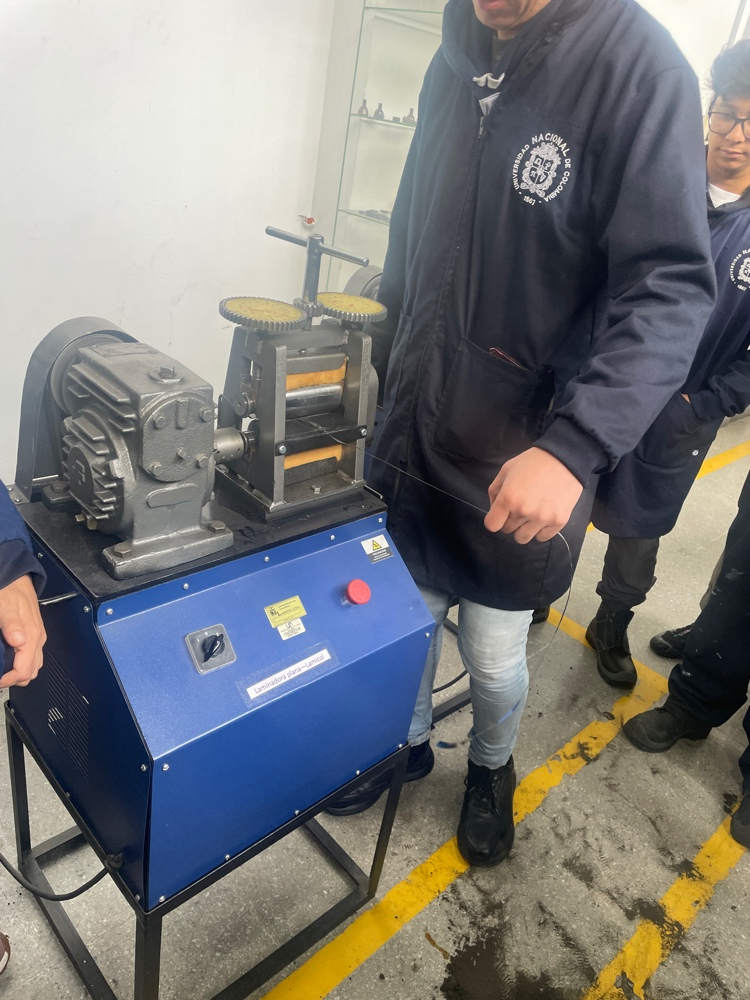
\includegraphics[width=0.60\columnwidth,keepaspectratio]{LaminadoraPlana.png}
\caption{Laminadora electromecánica plana empleada en el laboratorio.}
\label{fig:laminadora_equipo}
\end{figure}

\subsubsection{Instrumentos de Medición e Insumos}
\begin{itemize}
    \item Calibrador vernier (pie de rey): Resolución de $0.05\text{ mm}$ para registrar anchos y longitudes moderadas.
    \item Micrómetro de exteriores: Rango $0-25\text{ mm}$ con resolución de $0.001\text{ mm}$, empleado para medir con precisión diámetros iniciales y espesores delgados.
    \item Regla metálica graduada y cinta métrica: Utilizadas para medir probetas alargadas ($L > 400\text{ mm}$).
    \item Aceite lubricante: Aplicado sobre las caras de contacto para reducir la fricción y el desgaste entre la probeta y los rodillos.
\end{itemize}

\begin{figure}[h]
\centering
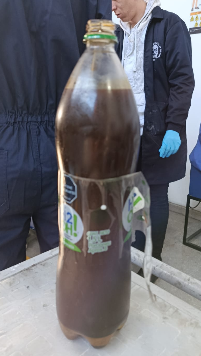
\includegraphics[width=0.40\columnwidth,keepaspectratio]{Lubricante.png}
\caption{Lubricante utilizado.}
\label{fig:lubricante_aceite}
\end{figure}

\subsection{Normas de Seguridad}
Durante la sesión se cumplieron estrictamente las siguientes medidas:
\begin{itemize}
    \item Verificación del pulsador de parada de emergencia antes de operar.
    \item No acercar las manos a los rodillos en movimiento durante el paso del material.
    \item Uso obligatorio de gafas de seguridad y ropa de trabajo adecuada.
    \item Manipulación y medición de las probetas únicamente con el equipo totalmente detenido.
\end{itemize}

\subsection{Procedimiento Paso a Paso}
\begin{enumerate}
    \item \textbf{Identificación y medidas iniciales (Pase 0):} Marcado de las probetas y medición de su longitud inicial $L_0$ y diámetro inicial $d_0$.
    \item \textbf{Ajuste del entrehierro:} Calibración de la separación entre rodillos para lograr una reducción inicial moderada y segura.
    \item \textbf{Aplicación de lubricante:} Impregnación de una fina capa de aceite en la probeta para suavizar el paso y disminuir la fricción.
    \item \textbf{Pase de laminación:} Introducción de la probeta entre los rodillos giratorios, recibiendo la pieza en la bandeja de salida.
    
    \begin{figure}[h]
    \centering
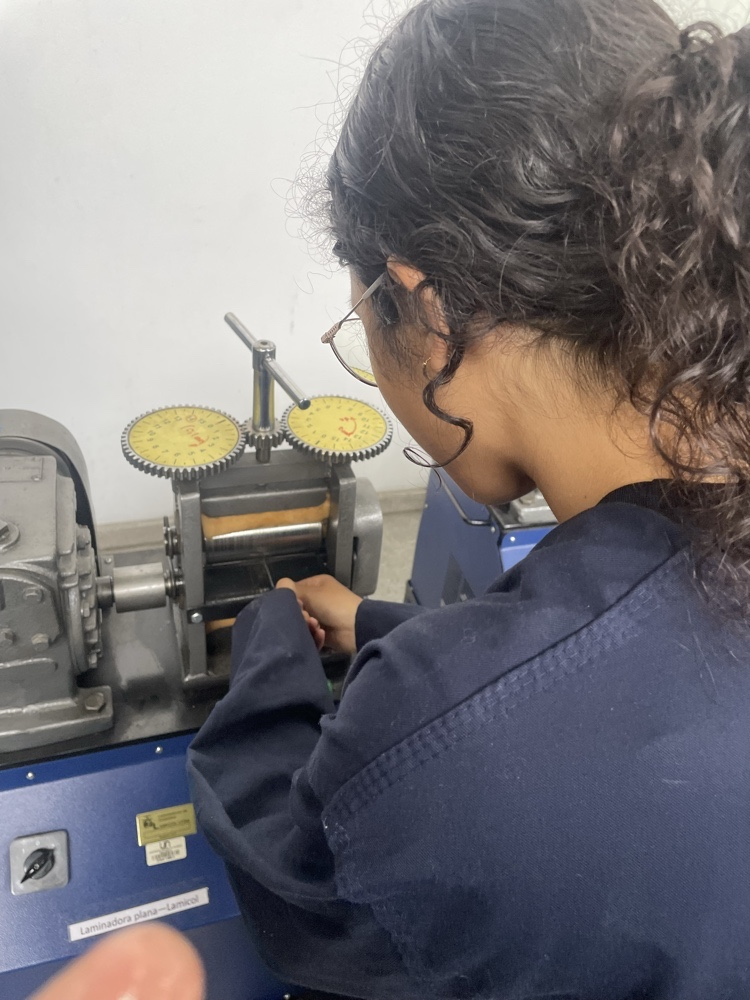
\includegraphics[width=0.60\columnwidth, keepaspectratio]{Laminando.png}
    \caption{Operación de alimentación y guiado de la probeta entre los rodillos.}
    \label{fig:laminando_proceso}
    \end{figure}
    
    \item \textbf{Medición y registro:} Con la máquina detenida, medición de longitud $L$, ancho $b$ y espesor $h$, anotando observaciones sobre curvatura, calentamiento y facilidad de paso.
    \item \textbf{Pases sucesivos:} Repetición del procedimiento ajustando los rodillos hacia un espesor menor en cada ciclo, hasta alcanzar el límite práctico del material o de la máquina.
\end{enumerate}


\section{Datos Experimentales y Cálculos}
En las Tablas~\ref{tab:datos_aluminio}, \ref{tab:datos_cobre} y \ref{tab:datos_acero_inox} se consolidan las dimensiones registradas durante la práctica para cada una de las pasadas de laminación realizadas sobre las probetas de aleación de aluminio, aleación de cobre y acero inoxidable.

\begin{table*}[t]
\centering
\caption{Registro experimental y cálculos de proceso para la probeta de Aleación de Aluminio}
\label{tab:datos_aluminio}
\footnotesize
\setlength{\tabcolsep}{3.5pt}
\renewcommand{\arraystretch}{1.15}
\begin{tabularx}{\textwidth}{c c c c c c c c >{\raggedright\arraybackslash}X}
\toprule
\textbf{Pase} & \makecell{\textbf{Longitud}\\\textbf{$L$ [mm]}} & \makecell{\textbf{Ancho}\\\textbf{$b$ [mm]}} & \makecell{\textbf{Espesor}\\\textbf{$h$ [mm]}} & \makecell{\textbf{Área}\\\textbf{$A$ [mm$^2$]}} & \textbf{\%Rh} & \textbf{\%El} & \textbf{\%CW} & \textbf{Observaciones experimentales y morfología} \\
\midrule
0 & 167.40 & 3.20 ($d_0$) & 3.20 ($d_0$) & 8.04 & 0.00\% & 0.00\% & 0.00\% & Probeta cilíndrica inicial lisa, sin imperfecciones visibles. \\ \addlinespace[3.5pt]
1 & 174.50 & 3.85 & 2.10 & 8.09 & 34.38\% & 4.24\% & $\sim 0.00\%$ & Transición a sección achatada; combado longitudinal; lubricación con aceite. \\ \addlinespace[3.5pt]
2 & 178.30 & 3.60 & 1.65 & 5.94 & 48.44\% & 6.51\% & 26.12\% & Ensanchamiento lateral; ondulacion; moderada resistencia plástica. \\ \addlinespace[3.5pt]
3 & 210.00 & 3.40 & 1.30 & 4.42 & 59.38\% & 25.45\% & 45.02\% & Notorio avance en elongación longitudinal; endurecimiento perceptible. \\ \addlinespace[3.5pt]
4 & 265.00 & 3.23 & 1.00 & 3.23 & 68.75\% & 58.30\% & 59.83\% & Bordes con ligera curvatura; sección transversal uniforme. \\ \addlinespace[3.5pt]
5 & 412.00 & 3.80 & 0.50 & 1.90 & 84.38\% & 146.12\% & 76.37\% & Cinta delgada y maleable; ondulacion generalizado; aplanada manualmente en mesa. \\ \addlinespace[3.5pt]
6 & 2310.00 & 5.80 & 0.10 & 0.58 & 96.88\% & 1279.93\% & 92.79\% & Espesor medido con micrómetro; rodillos en tope; cinta continua rizada final. \\
\bottomrule
\end{tabularx}
\end{table*}

\begin{table*}[t]
\centering
\caption{Registro experimental y cálculos de proceso para la probeta de Aleación de Cobre}
\label{tab:datos_cobre}
\footnotesize
\setlength{\tabcolsep}{3.5pt}
\renewcommand{\arraystretch}{1.15}
\begin{tabularx}{\textwidth}{c c c c c c c c >{\raggedright\arraybackslash}X}
\toprule
\textbf{Pase} & \makecell{\textbf{Longitud}\\\textbf{$L$ [mm]}} & \makecell{\textbf{Ancho}\\\textbf{$b$ [mm]}} & \makecell{\textbf{Espesor}\\\textbf{$h$ [mm]}} & \makecell{\textbf{Área}\\\textbf{$A$ [mm$^2$]}} & \textbf{\%Rh} & \textbf{\%El} & \textbf{\%CW} & \textbf{Observaciones experimentales y morfología} \\
\midrule
0 & 162.85 & 2.35 ($d_0$) & 2.35 ($d_0$) & 4.34 & 0.00\% & 0.00\% & 0.00\% & Varilla cilíndrica lisa de aleación de cobre, sin defectos previos. \\ \addlinespace[3.5pt]
1 & 164.10 & 2.79 & 1.90 & 5.30 & 19.15\% & 0.77\% & $\sim 0.00\%$ & Reducción inicial moderada; ligero calentamiento al tacto; aumento de rigidez. \\ \addlinespace[3.5pt]
2 & 180.00 & 3.20 & 1.40 & 4.48 & 40.43\% & 10.53\% & $\sim 0.00\%$ & Curvatura residual al salir de los rodillos; deformación con mayor resistencia. \\ \addlinespace[3.5pt]
3 & 258.00 & 4.00 & 0.60 & 2.40 & 74.47\% & 58.43\% & 44.70\% & Probeta sale bastante caliente por la deformación; enfriamiento rápido en mesa. \\ \addlinespace[3.5pt]
4 & 445.00 & 4.85 & 0.324 & 1.57 & 86.21\% & 173.26\% & 63.82\% & Espesor medido con micrómetro; cinta adelgazada con alta rigidez elástica. \\
\bottomrule
\end{tabularx}
\end{table*}

\begin{table*}[t]
\centering
\caption{Registro experimental y cálculos de proceso para la probeta de Acero Inoxidable}
\label{tab:datos_acero_inox}
\footnotesize
\setlength{\tabcolsep}{3.5pt}
\renewcommand{\arraystretch}{1.15}
\begin{tabularx}{\textwidth}{c c c c c c c c >{\raggedright\arraybackslash}X}
\toprule
\textbf{Pase} & \makecell{\textbf{Longitud}\\\textbf{$L$ [mm]}} & \makecell{\textbf{Ancho}\\\textbf{$b$ [mm]}} & \makecell{\textbf{Espesor}\\\textbf{$h$ [mm]}} & \makecell{\textbf{Área}\\\textbf{$A$ [mm$^2$]}} & \textbf{\%Rh} & \textbf{\%El} & \textbf{\%CW} & \textbf{Observaciones experimentales y morfología} \\
\midrule
0 & 190.00 & 2.374 ($d_0$) & 2.374 ($d_0$) & 4.43 & 0.00\% & 0.00\% & 0.00\% & Probeta cilíndrica inicial de acero inoxidable, medida con micrómetro y cinta métrica. \\ \addlinespace[3.5pt]
1 & 218.00 & 2.496 & 2.052 & 5.12 & 13.56\% & 14.74\% & $\sim 0.00\%$ & Reducción inicial moderada; ligero endurecimiento perceptible; curvatura suave al salir de rodillos. \\ \addlinespace[3.5pt]
2 & 255.00 & 2.771 & 1.450 & 4.02 & 38.92\% & 34.21\% & 9.23\% & Deformación intermedia progresiva; incremento del esfuerzo requerido y calentamiento al tacto. \\ \addlinespace[3.5pt]
3 & 309.00 & 3.515 & 0.906 & 3.18 & 61.84\% & 62.63\% & 28.05\% & Probeta notablemente caliente por la deformación plástica; aumento severo de rigidez elástica. \\ \addlinespace[3.5pt]
4 & 565.00 & 4.773 & 0.380 & 1.81 & 83.99\% & 197.37\% & 59.02\% & Cinta delgada; ensanchamiento pronunciado; ondulaciones ligeras en los bordes libres. \\ \addlinespace[3.5pt]
5 & 810.00 & 4.791 & 0.264 & 1.26 & 88.88\% & 326.32\% & 71.43\% & Cinta final delgada; espesor y ancho verificados con micrómetro; longitud con cinta métrica; alta acritud. \\
\bottomrule
\end{tabularx}
\end{table*}

\subsection{Memoria de Cálculos y Fórmulas Aplicadas}
Para la obtención de las columnas calculadas en las tablas se emplearon directamente las ecuaciones expuestas en el fundamento teórico (Sección~III):

\subsubsection{Cálculo de Áreas Transversales}
En el estado inicial (Pase 0), la probeta posee geometría cilíndrica de diámetro $d_0$, por lo que su área transversal inicial ($A_0$) se determinó mediante la ecuación~(\ref{eq:area_cilindro}).

A partir del primer pase, al ser aplastada entre los rodillos, la pieza adquiere una sección transversal aproximadamente rectangular caracterizada por su ancho $b$ y su espesor $h$, calculándose el área ($A$) con la ecuación~(\ref{eq:area_rectangulo}).


\subsubsection{Reducción de Espesor (\%Rh)}
Mide la magnitud del calado impuesto por los rodillos en cada pasada respecto al espesor inicial de la probeta, de acuerdo con la ecuación~(\ref{eq:rh}).


\subsubsection{Elongación Longitudinal (\%El)}
Cuantifica el alargamiento porcentual de la pieza a lo largo de la dirección de avance como consecuencia de la reducción del espesor, calculada mediante la ecuación~(\ref{eq:elongacion}).


\subsubsection{Porcentaje de Trabajo en Frío (\%CW)}
Representa la deformación plástica acumulada calculada mediante la ecuación~(\ref{eq:cw}). Cabe señalar que en las primeras pasadas se reporta un valor de $\sim 0.00\%$ debido a la transición geométrica de sección circular a rectangular; al aproximar el área transversal simplemente como $A = b \cdot h$, se sobreestima el área real por no considerar los bordes curvados u ovalados de la probeta, lo que arroja matemáticamente una reducción de área nula o ligeramente negativa a pesar del alargamiento registrado.
\subsubsection{Ensanchamiento Lateral (\%\texorpdfstring{$\Delta$}{D}b)}
Evalúa el flujo plástico transversal en los bordes libres según la ecuación~(\ref{eq:delta_b}).
\subsubsection{Deformación Verdadera (\texorpdfstring{$\varepsilon$}{e})}
Describe la deformación plástica real acumulada según la ecuación~(\ref{eq:deformacion}). Los valores calculados se presentan en la Tabla~\ref{tab:deformacion_verdadera}.

\begin{table}[h]
\centering
\caption{Evolución de la Deformación Verdadera ($\varepsilon$) por Pase}
\label{tab:deformacion_verdadera}
\footnotesize
\renewcommand{\arraystretch}{1.15}
\begin{tabular}{c c c c}
\toprule
\textbf{Pase} & \textbf{$\varepsilon$ Aluminio} & \textbf{$\varepsilon$ Cobre} & \textbf{$\varepsilon$ Inox} \\
\midrule
1 & 0.421 & 0.213 & 0.146 \\ \addlinespace[2.5pt]
2 & 0.662 & 0.518 & 0.493 \\ \addlinespace[2.5pt]
3 & 0.901 & 1.365 & 0.963 \\ \addlinespace[2.5pt]
4 & 1.163 & 1.981 & 1.832 \\ \addlinespace[2.5pt]
5 & 1.856 & ---   & 2.196 \\ \addlinespace[2.5pt]
6 & 3.466 & ---   & ---   \\
\bottomrule
\end{tabular}
\end{table}

\subsubsection{Verificación de la Constancia de Volumen}
El principio de conservación de volumen ($V = L \cdot A = \text{cte}$, ec.~\ref{eq:volumen}) se evaluó calculando el volumen inicial ($V_0 = A_0 L_0$) y final ($V_f = A_f L_f$) de cada probeta:
\begin{itemize}\setlength{\itemsep}{1pt}\setlength{\parskip}{0pt}
    \item \textbf{Aleación de Aluminio:} $V_0 = 1345.90\text{ mm}^3$ y $V_f = 1339.80\text{ mm}^3$ (Pase~6). Variación: $-0.45\%$.
    \item \textbf{Aleación de Cobre:} $V_0 = 706.77\text{ mm}^3$ y $V_f = 698.65\text{ mm}^3$ (Pase~4). Variación: $-1.15\%$.
    \item \textbf{Acero Inoxidable:} $V_0 = 841.01\text{ mm}^3$ y $V_f = 1024.51\text{ mm}^3$ (Pase~5). Variación: $+21.82\%$.
\end{itemize}
En las probetas de aluminio y cobre se verifica de manera rigurosa la incompresibilidad plástica ($|\Delta V| \le 1.15\%$). En el caso del acero inoxidable, la variación volumétrica ($+21.82\%$) se debe a las ondulaciones en los bordes de la cinta delgada, lo que incrementa el área transversal aparente registrada durante las mediciones.

\section{Gráficas del Proceso}
A continuación se grafica el porcentaje de trabajo en frío en función del número de pases, el porcentaje de elongación longitudinal vs. número de pases, la reducción porcentual de espesor y la deformación verdadera ($\varepsilon$). En las Figuras~\ref{fig:grafica_cw}, \ref{fig:grafica_elongacion}, \ref{fig:grafica_rh} y \ref{fig:grafica_deformacion} se presentan las curvas experimentales correspondientes calculadas a partir de las dimensiones de las probetas.
\begin{figure}[h]
\centering
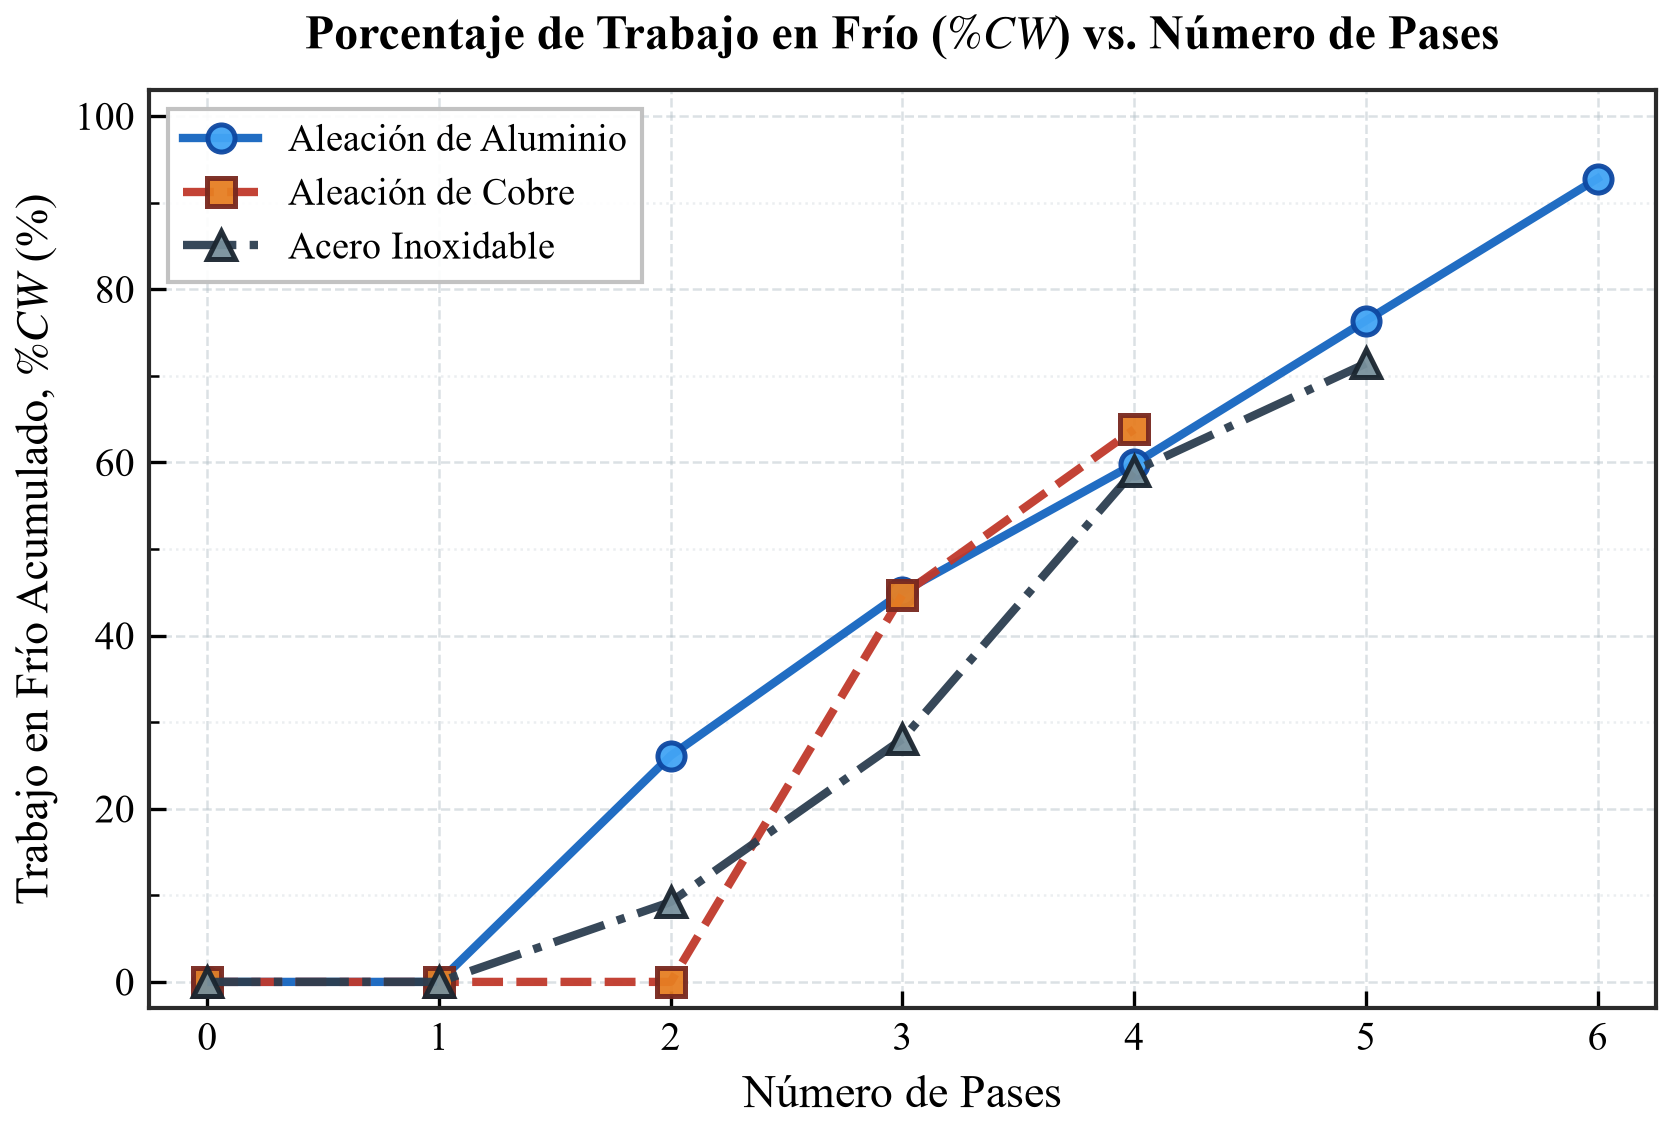
\includegraphics[width=\columnwidth,keepaspectratio]{grafica_cw.png}
\caption{Porcentaje de trabajo en frío (\%CW) en función del número de pases para cada material.}
\label{fig:grafica_cw}
\end{figure}

\begin{figure}[h]
\centering
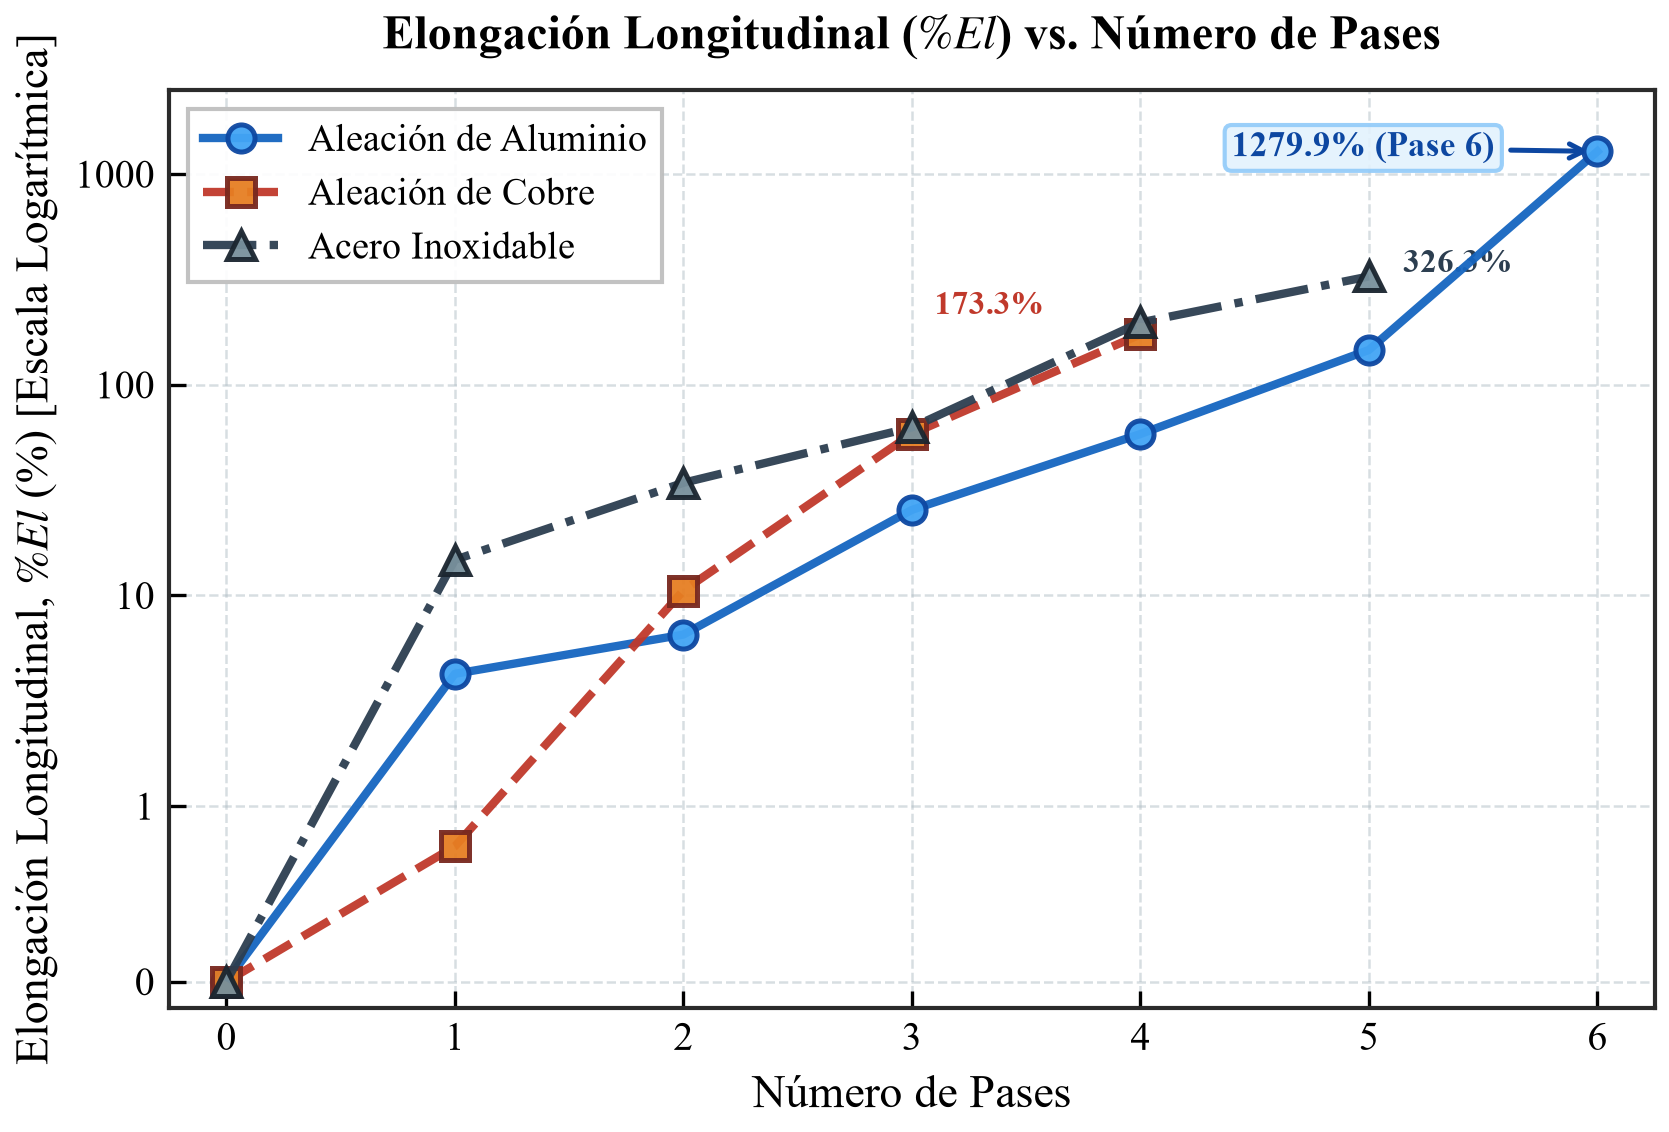
\includegraphics[width=\columnwidth,keepaspectratio]{grafica_elongacion.png}
\caption{Porcentaje de elongación longitudinal (\%El) en función del número de pases.}
\label{fig:grafica_elongacion}
\end{figure}

\begin{figure}[h]
\centering
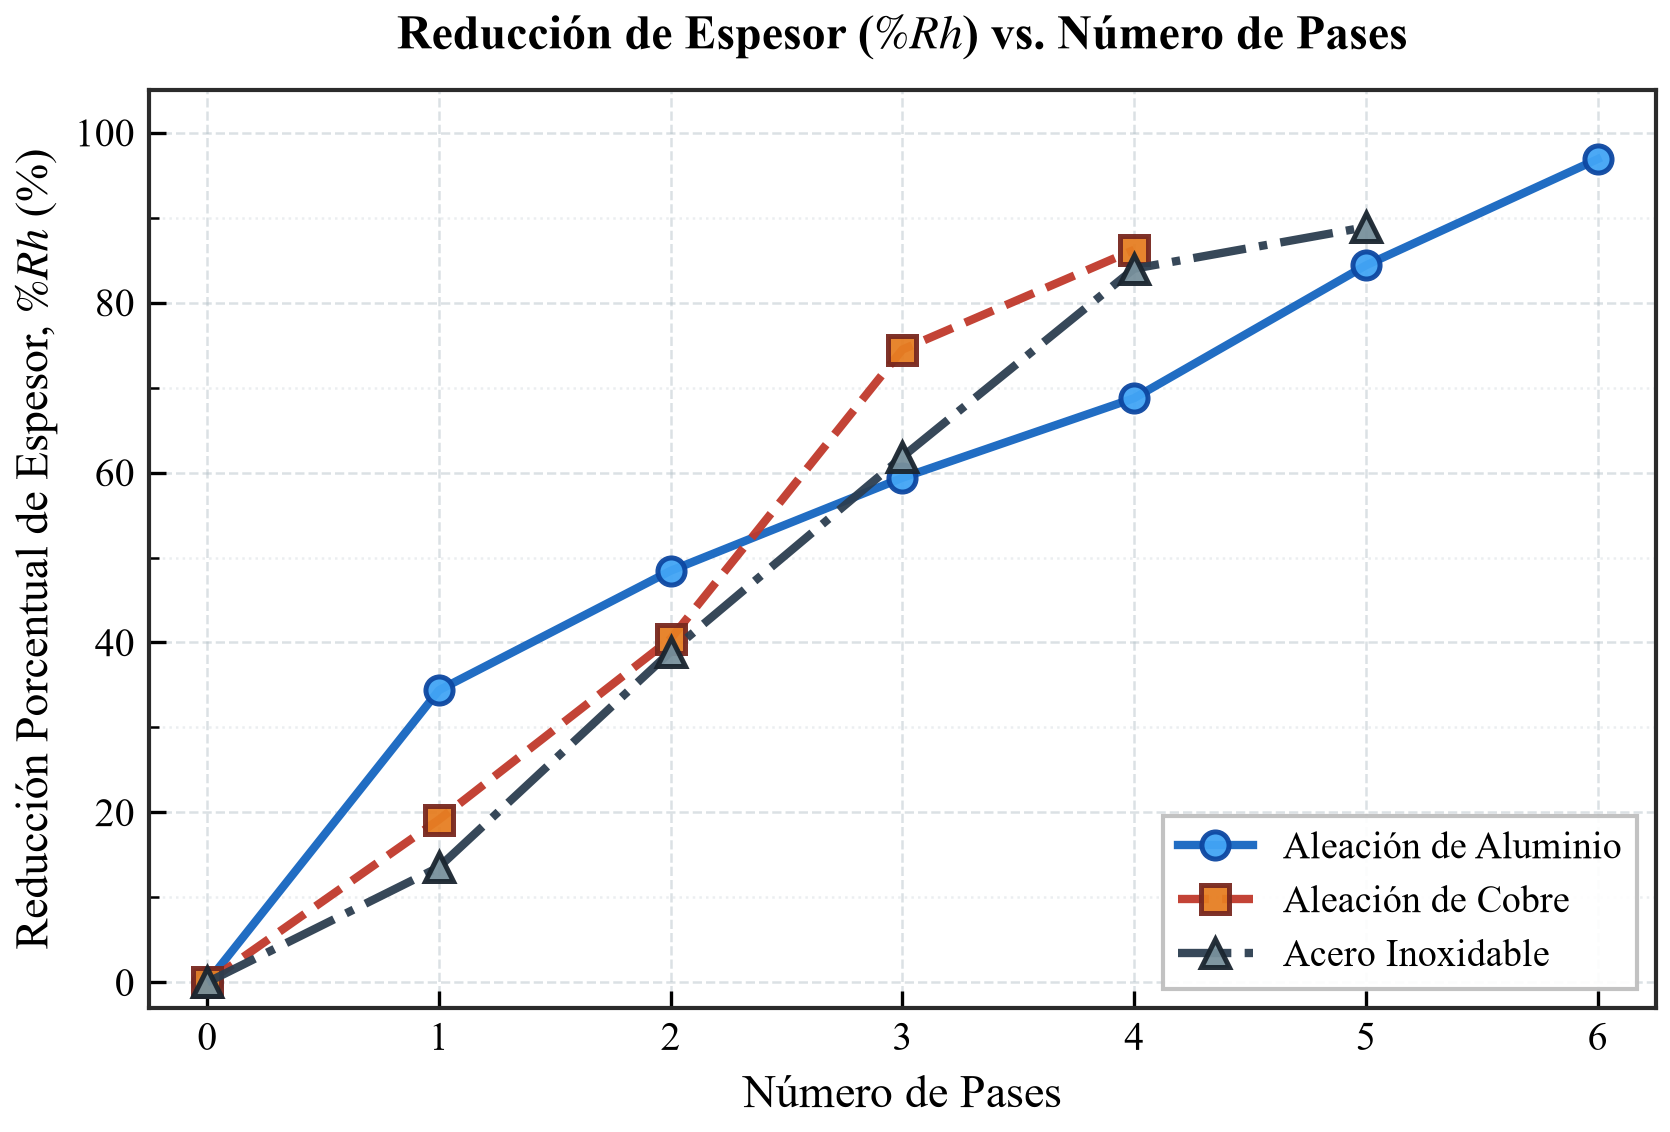
\includegraphics[width=\columnwidth,keepaspectratio]{grafica_rh.png}
\caption{Comparación de la evolución geométrica de reducción de espesor (\%Rh) en función del número de pases.}
\label{fig:grafica_rh}
\end{figure}

\begin{figure}[H]
\centering
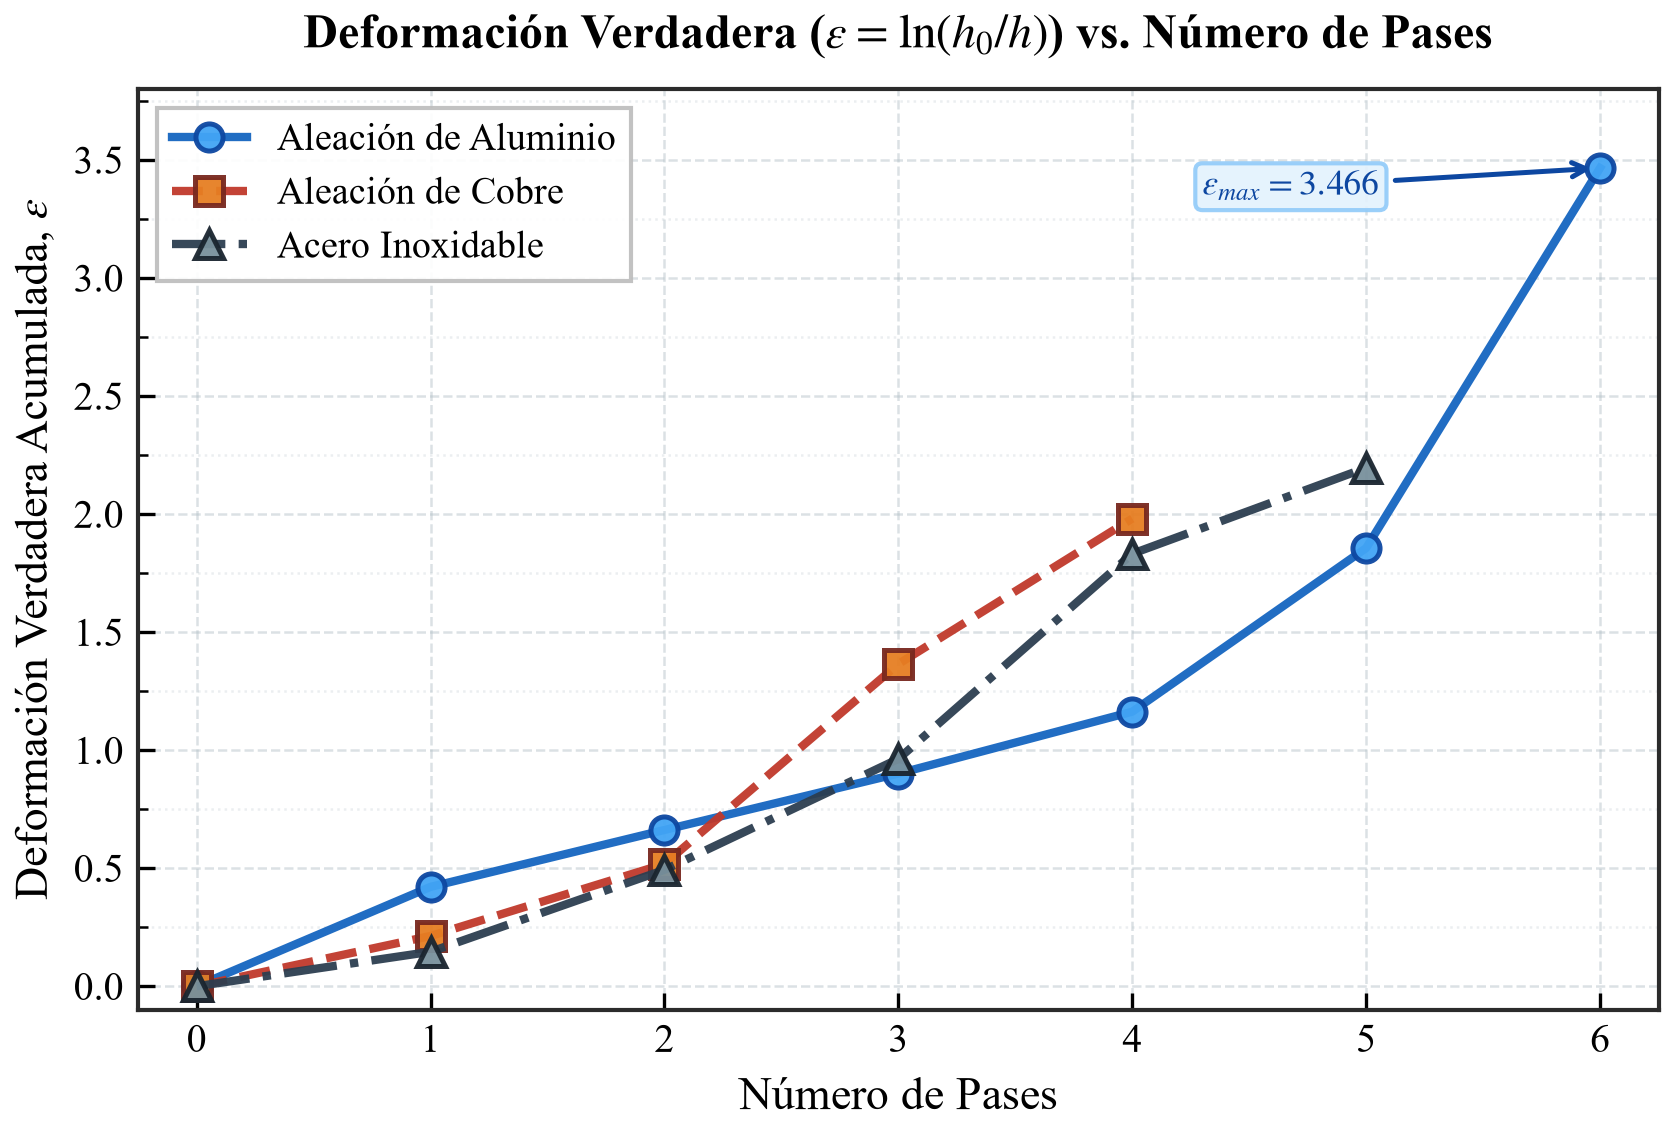
\includegraphics[width=\columnwidth,keepaspectratio]{grafica_deformacion.png}
\caption{Evolución de la deformación verdadera ($\varepsilon$) en función del número de pases.}
\label{fig:grafica_deformacion}
\end{figure}

\section{Registro Fotográfico del Proceso}
En concordancia con las indicaciones del laboratorio, a continuación se presenta el registro visual individual de las probetas durante el ensayo, documentando la evolución morfológica macroscópica para la aleación de aluminio, la aleación de cobre y el acero inoxidable en sus estados inicial (Figuras~\ref{fig:al_ini}--\ref{fig:ai_ini}), intermedio (Figuras~\ref{fig:al_med}--\ref{fig:ai_med}) y final (Figuras~\ref{fig:al_fin}--\ref{fig:ai_fin}):

\subsection{Estado Inicial}
\begin{figure}[H]
\centering
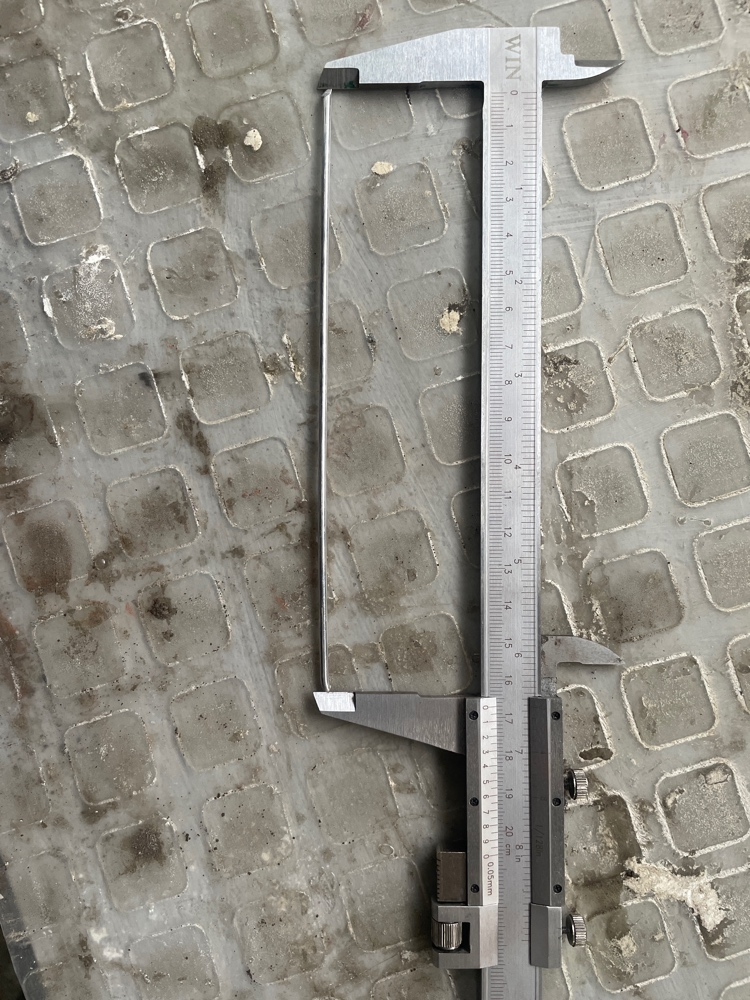
\includegraphics[width=0.85\columnwidth,keepaspectratio]{AluminioP0.png}
\caption{Aleación de aluminio en estado inicial (Pase~0).}
\label{fig:al_ini}
\end{figure}

\begin{figure}[H]
\centering
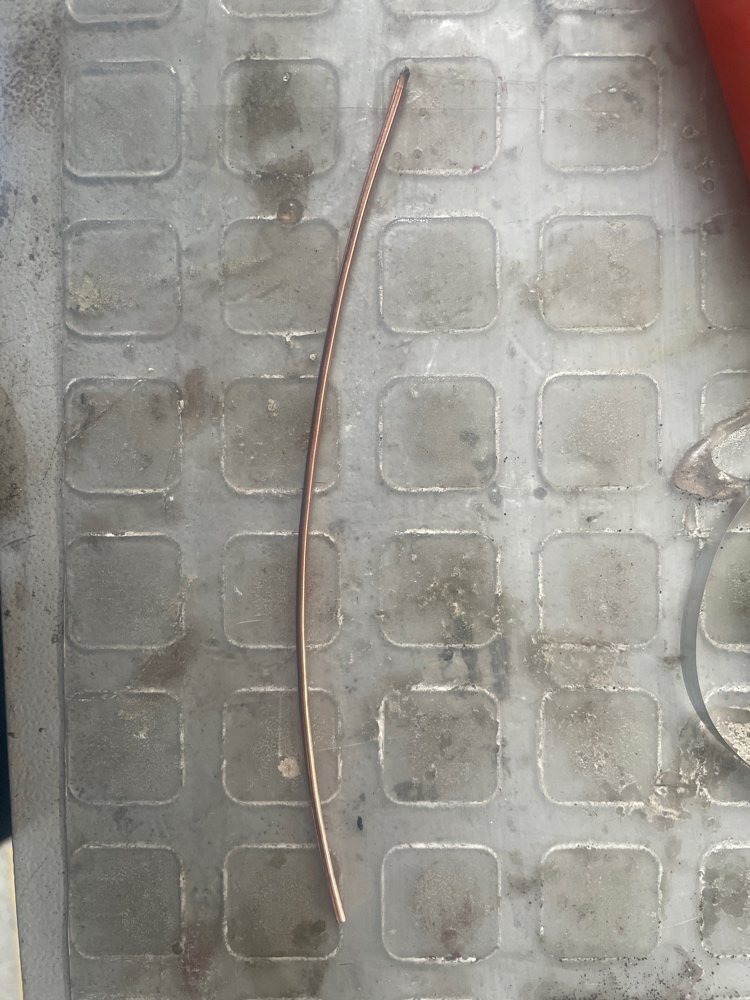
\includegraphics[width=0.85\columnwidth,keepaspectratio]{CobreP0.png}
\caption{Aleación de cobre en estado inicial (Pase~0).}
\label{fig:cu_ini}
\end{figure}

\begin{figure}[H]
\centering
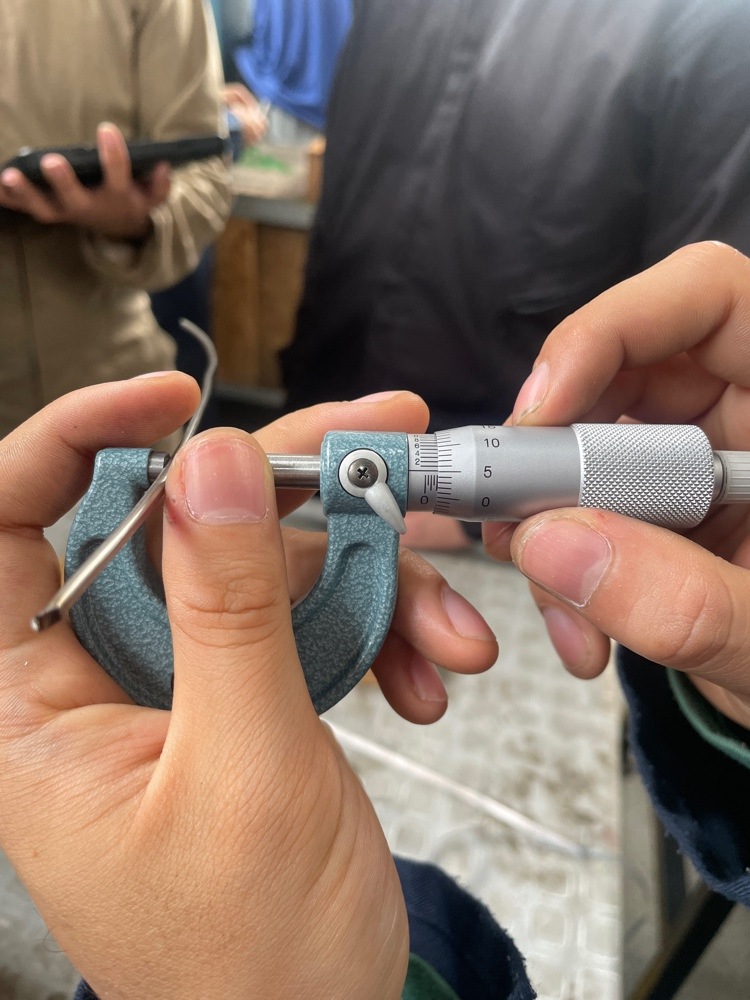
\includegraphics[width=0.85\columnwidth,keepaspectratio]{AceroInoxidableP1.png}
\caption{Acero inoxidable en estado inicial (Pase~0).}
\label{fig:ai_ini}
\end{figure}

\subsection{Estado Intermedio}
\begin{figure}[H]
\centering
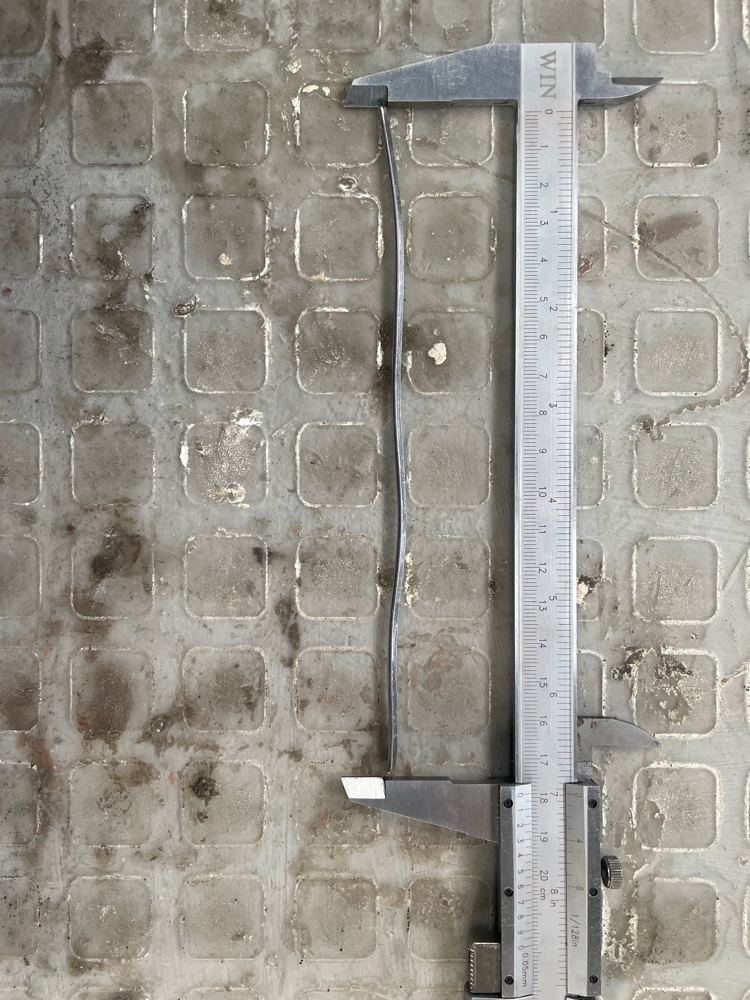
\includegraphics[width=0.85\columnwidth,keepaspectratio]{AluminioP2.png}
\caption{Aleación de aluminio en estado intermedio (Pase~2).}
\label{fig:al_med}
\end{figure}

\begin{figure}[H]
\centering
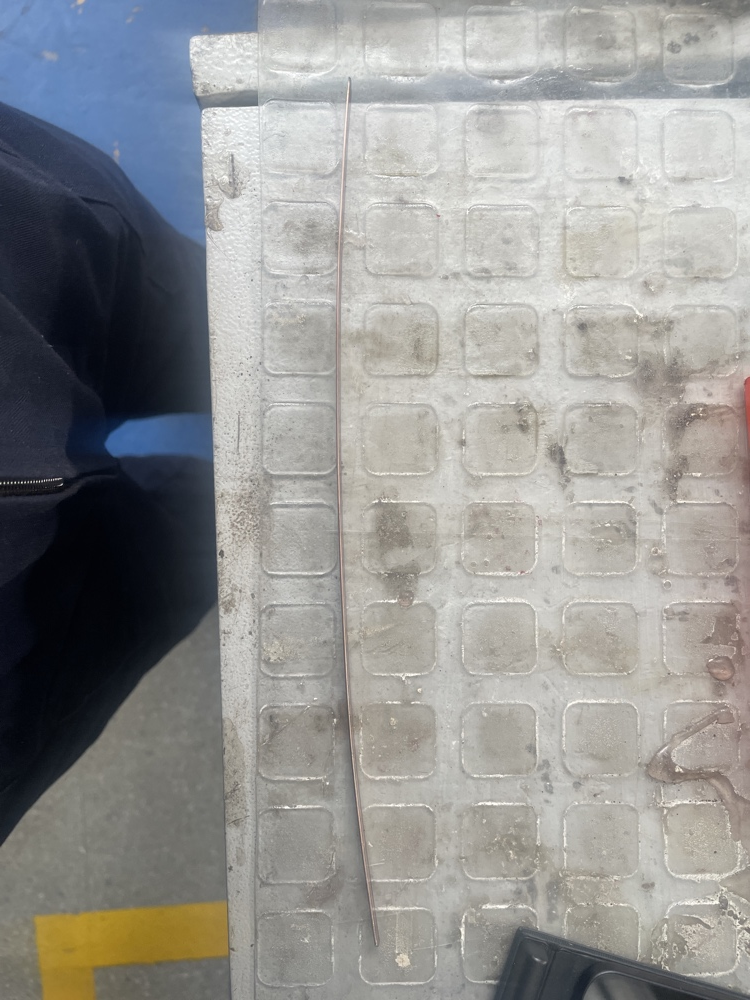
\includegraphics[width=0.85\columnwidth,keepaspectratio]{CobreP3.png}
\caption{Aleación de cobre en estado intermedio (Pase~3).}
\label{fig:cu_med}
\end{figure}

\begin{figure}[H]
\centering
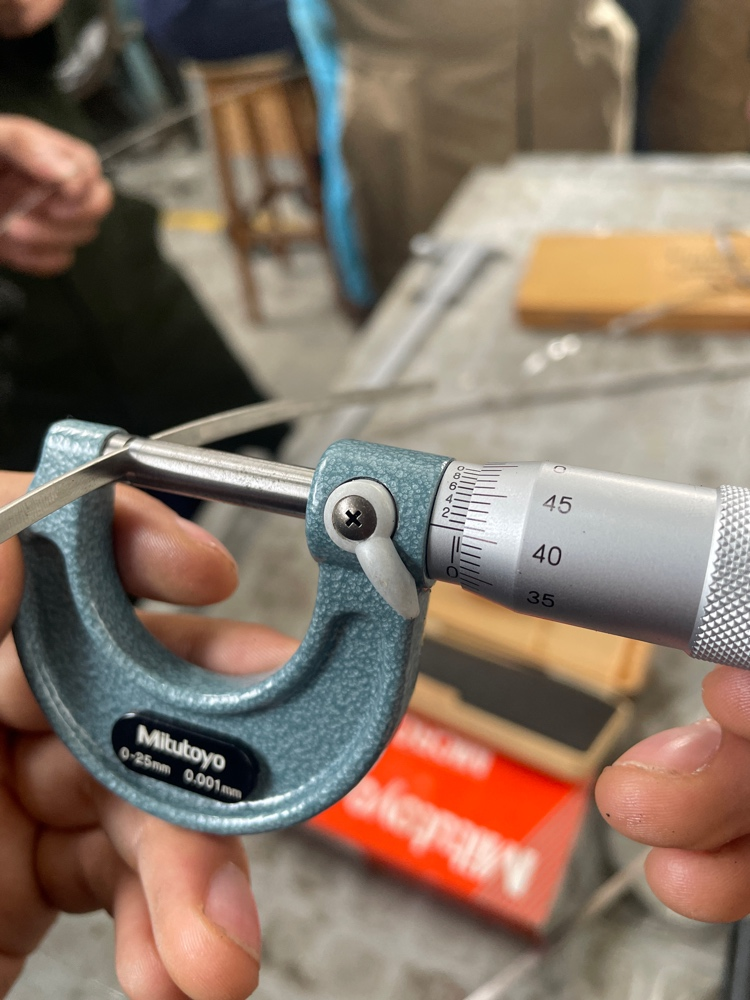
\includegraphics[width=0.85\columnwidth,keepaspectratio]{AceroInoxidableP3.png}
\caption{Acero inoxidable en estado intermedio (Pase~3).}
\label{fig:ai_med}
\end{figure}

\subsection{Estado Final}
\begin{figure}[H]
\centering
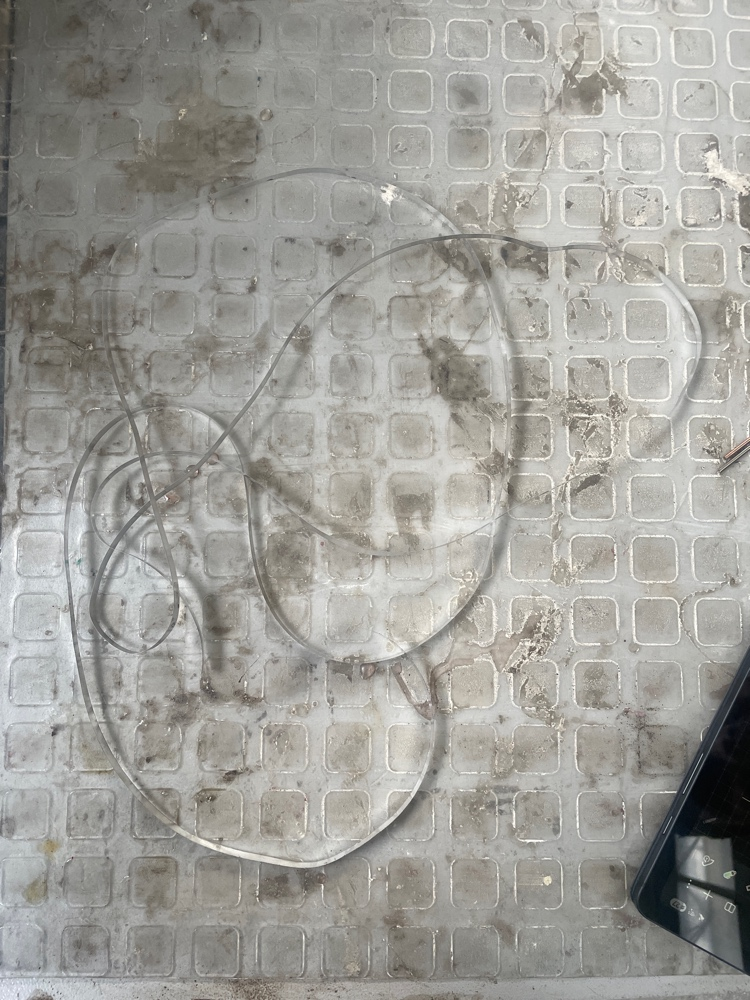
\includegraphics[width=0.85\columnwidth,keepaspectratio]{AluminioFinal.png}
\caption{Aleación de aluminio en estado final tras 6 pases de laminación.}
\label{fig:al_fin}
\end{figure}

\begin{figure}[H]
\centering
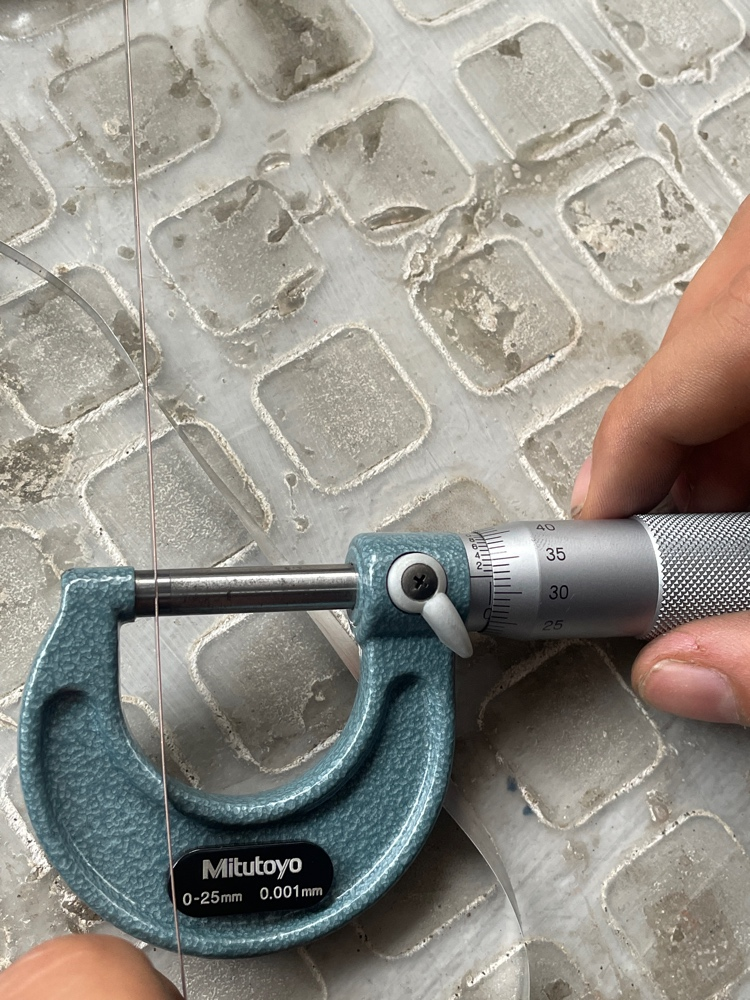
\includegraphics[width=0.85\columnwidth,keepaspectratio]{CobreP4.png}
\caption{Aleación de cobre en estado final tras 4 pases de laminación.}
\label{fig:cu_fin}
\end{figure}

\begin{figure}[H]
\centering
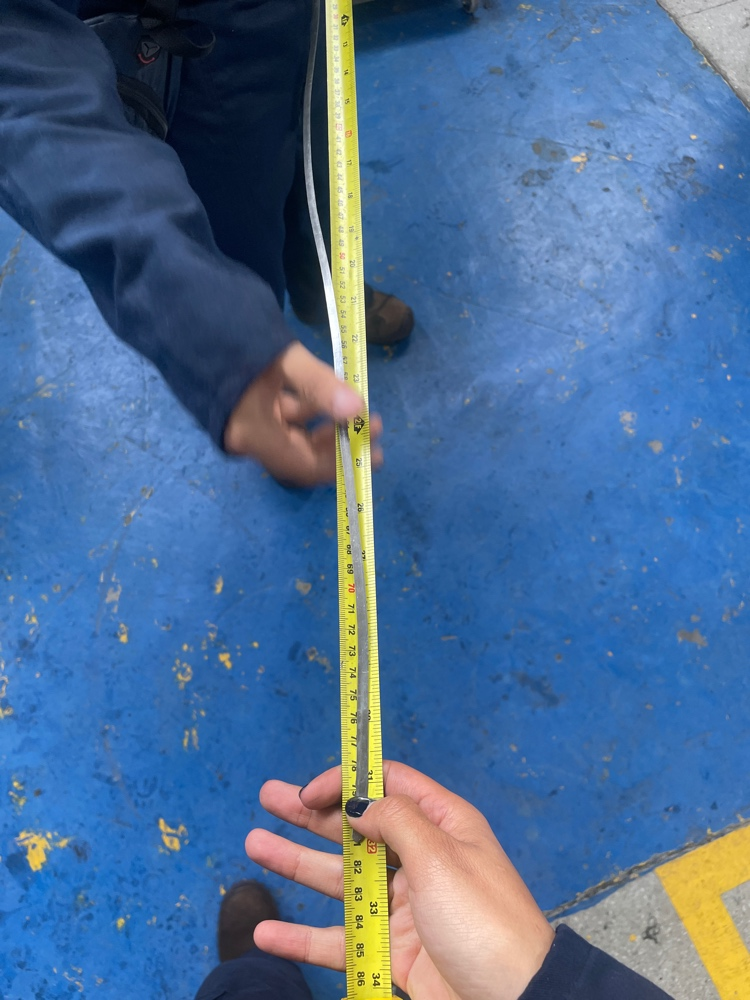
\includegraphics[width=0.85\columnwidth,keepaspectratio]{AceroInoxidableP5.png}
\caption{Acero inoxidable en estado final tras 5 pases de laminación.}
\label{fig:ai_fin}
\end{figure}

\section{Discusión de Resultados}
La discusión se organiza respondiendo de forma clara y directa a las preguntas establecidas en las indicaciones del laboratorio:

\subsection{Factores que Explican las Diferencias en el Comportamiento Plástico}
\textit{¿Qué factores explican las diferencias en el comportamiento plástico entre aluminio, cobre y acero inoxidable?}

Las diferencias se deben principalmente a la composición química y la facilidad con la que cada metal permite el movimiento de sus dislocaciones internas durante la deformación en frío. El aluminio ensayado posee una alta ductilidad natural y baja resistencia mecánica inicial, lo que le permite deformarse con facilidad y admitir reducciones severas sin romperse. La aleación de cobre contiene elementos aleantes que aumentan su resistencia mecánica inicial y provocan un endurecimiento progresivo sensible, haciendo que la pieza gane rigidez rápidamente y se caliente al ser deformada. Por su parte, el acero inoxidable cuenta con una alta cantidad de elementos de aleación como cromo y níquel; esto restringe fuertemente la deformación plástica y genera una tasa de endurecimiento muy alta, requiriendo mucha más fuerza en la máquina y provocando calentamiento y ondulaciones en bordes.

\subsection{Relación con la Estructura Cristalina y la Composición}
\textit{¿Cómo se relaciona el comportamiento observado con la estructura cristalina y la composición de cada material?}

Tanto el aluminio como el cobre y el acero inoxidable poseen una estructura cristalina cúbica centrada en las caras (FCC). Esta estructura cuenta teóricamente con numerosos planos de deslizamiento, lo que les confiere buena deformabilidad. Sin embargo, su comportamiento real varía por efecto de su composición: en el aluminio comercial, las dislocaciones se mueven libremente, permitiendo una gran deformación continua. En la aleación de cobre y en el acero inoxidable, los átomos de los elementos aleantes distorsionan la red cristalina y frenan el avance de las dislocaciones, produciendo un endurecimiento por deformación mucho más severo que limita el número de pases posibles.

\subsection{Material con Mayor Deformabilidad y Mayor Resistencia}
\textit{¿Qué material presentó mayor deformabilidad y cuál mayor resistencia al laminado? Justifique con los datos experimentales.}
\begin{itemize}
    \item \textbf{Mayor deformabilidad:} El \textbf{Aluminio}. Fue el único material que completó los seis pases programados sin presentar grietas ni fracturas. Logró una elongación longitudinal extraordinaria del $1279.93\%$ (pasando de $167.40\text{ mm}$ a $2310.00\text{ mm}$) y una reducción de espesor del $96.88\%$ (de $3.20\text{ mm}$ a $0.10\text{ mm}$), alcanzando un trabajo en frío de $\%CW = 92.79\%$.
    \item \textbf{Mayor resistencia al laminado:} El \textbf{Acero Inoxidable}. Presentó la mayor resistencia al avance de los rodillos desde los primeros pases. Tras cinco pasadas acumuló un $71.43\%$ de trabajo en frío y un espesor de $0.264\text{ mm}$, momento en el que la rigidez del material y la aparición de ondulaciones en los bordes hicieron desaconsejable continuar para no sobrecargar el equipo.
\end{itemize}

\subsection{Ensanchamiento Lateral}
\textit{¿Se observó ensanchamiento lateral? ¿Fue igual en todos los materiales?}

Sí, se observó ensanchamiento lateral en los tres materiales, pero no fue igual en todos ni de la misma proporción. En el acero inoxidable el ancho aumentó de $2.374\text{ mm}$ a $4.791\text{ mm}$ ($+101.81\%$), en la aleación de cobre pasó de $2.35\text{ mm}$ a $4.85\text{ mm}$ ($+106.38\%$), y en el aluminio pasó de $3.20\text{ mm}$ a $5.80\text{ mm}$ ($+81.25\%$). (Si para el acero inoxidable se evalúa el ensanchamiento tomando como referencia el ancho tras el primer pase plano, $b_1 = 2.496\text{ mm}$, el incremento resultante es de $+91.95\%$).

A pesar de estos aumentos en el ancho, el flujo del material fue predominantemente longitudinal (en el aluminio la longitud creció más del $1200\%$, mientras el ancho solo creció $81\%$). Esto sucede porque la fricción en el arco de contacto entre los rodillos restringe la salida lateral del metal, obligándolo a fluir hacia adelante en el sentido del giro.

\subsection{Evidencia Experimental del Endurecimiento por Deformación}
\textit{¿Qué evidencia experimental sugiere endurecimiento por deformación?}

Durante el laboratorio se evidenció el endurecimiento por deformación a través de las siguientes observaciones:
\begin{enumerate}
    \item \textbf{Aumento de la rigidez manual:} Las probetas de cobre y acero inoxidable, que inicialmente se doblaban fácilmente con la mano, después de los pases 3 y 4 se volvieron muy duras y rígidas, siendo casi imposible flexionarlas manualmente.
    \item \textbf{Calentamiento de las probetas:} En los pases avanzados de la aleación de cobre y del acero inoxidable, las piezas salieron de los rodillos notablemente calientes al tacto, producto del trabajo mecánico disipado en forma de calor durante la deformación plástica en frío.
    \item \textbf{Mayor resistencia en los rodillos:} Cada nueva pasada requirió apretar más los husillos y ejerció mayor esfuerzo sobre el motor y los rodillos de la laminadora para lograr reducciones cada vez más pequeñas.
\end{enumerate}

\subsection{Defectos por Excesiva Reducción por Pase}
\textit{¿Qué defectos podrían aparecer si se incrementa demasiado la reducción por pase?}

Si se intenta reducir demasiado espesor en una sola pasada, pueden presentarse fallas graves:
\begin{itemize}
    \item \textbf{Acocodrilado:} Apertura longitudinal de la cinta en dos mitades por tensiones internas.
    \item \textbf{Agrietamiento en los bordes:} Fisuras transversales en las orillas de la lámina cuando el material agota su ductilidad.
    \item \textbf{Patinaje de los rodillos:} Si la reducción es muy grande, los rodillos no logran atrapar la pieza y patinan sobre su superficie, rayando el material.
    \item \textbf{Atascamiento del motor:} Sobrecarga mecánica en la caja reductora o en el motor por exceder la capacidad de fuerza del equipo.
\end{itemize}

\subsection{Variable de Proceso Más Importante}
\textit{¿Qué variable de proceso sería la más importante de controlar en esta práctica?}

La variable más importante es la \textbf{reducción de espesor por pase ($\Delta h$)}. Esta determina directamente la fuerza que soportan los rodillos, el nivel de endurecimiento del metal y la calidad superficial de la pieza. Una reducción moderada y progresiva garantiza que el material fluya de manera uniforme sin agrietarse, que los rodillos no patinen y que no se sobrecargue el tren motriz de la máquina.

\subsection{Aplicaciones Industriales de los Resultados}
\textit{¿Qué aplicaciones industriales pueden asociarse a los resultados observados?}
\begin{itemize}
    \item \textbf{Aleaciones de Aluminio:} Fabricación de papel de aluminio para empaques, latas para bebidas, aletas de radiadores y paneles para la industria automotriz y aeronáutica, donde se requiere máxima maleabilidad y ligereza.
    \item \textbf{Aleaciones de Cobre:} Producción de flejes, cintas y terminales para conductores eléctricos, tuberías e intercambiadores de calor, aprovechando su buena conductividad y su resistencia tras el conformado.
    \item \textbf{Acero Inoxidable:} Fabricación de láminas y flejes delgados para recipientes de la industria química, tanques de procesamiento de alimentos, utensilios de cocina e instrumental médico, donde se necesita alta resistencia mecánica y resistencia a la corrosión con acabado pulido.
\end{itemize}

\section{Conclusiones}
\begin{enumerate}
    \item Se verificó experimentalmente el principio de conservación de volumen en conformado plástico para las probetas de aluminio (variación neta de $-0.45\%$) y cobre (variación de $-1.15\%$), confirmando la incompresibilidad con márgenes inferiores al $2\%$; en el acero inoxidable se obtuvo una variación de $+21.82\%$ debida a las ondulaciones y curvaturas residuales en los bordes de la cinta delgada y posibles errores de medición.
    \item La respuesta al laminado dependió notablemente del tipo de material: el aluminio presentó la mayor ductilidad completando 6 pases sin fallar (alcanzando un $\%CW$ de $92.79\%$ y una elongación de $1279.93\%$), mientras que la aleación de cobre y el acero inoxidable presentaron un rápido endurecimiento que limitó su proceso a 4 y 5 pases respectivamente.
    \item La deformación plástica fue principalmente longitudinal debido a la restricción impuesta por el contacto de los rodillos, presentándose un ensanchamiento lateral secundario pero medible en los tres materiales ($81.25\%$ en aluminio, $106.38\%$ en cobre y $101.81\%$ en acero inoxidable respecto al estado inicial).
    \item El endurecimiento por deformación en frío se evidenció de manera directa en el incremento de rigidez al tacto, el calentamiento de las probetas durante el pase y la necesidad de aplicar mayor fuerza de apriete en la máquina para reducciones sucesivas.
    \item El control adecuado de la reducción por pase y la lubricación interfacial resultaron fundamentales para prevenir defectos como agrietamiento de bordes, ondulaciones y sobrecarga en el equipo de laminación.
\end{enumerate}

\begin{thebibliography}{00}

\bibitem{kalpakjian2014}
S.~Kalpakjian y S.~R.~Schmid, \emph{Manufactura, ingeniería y tecnología}, 7.ª~ed. México: Pearson Educación, 2014.

\bibitem{groover2020}
M.~P.~Groover, \emph{Fundamentos de manufactura moderna: materiales, procesos y sistemas}, 3.ª~ed. México: McGraw-Hill Interamericana, 2020.

\end{thebibliography}

\end{document}
